% INTRODUÇÃO-------------------------------------------------------------------

\chapter{Introdução}
\label{chap:introducao}

Este relatório descreve as atividades realizadas, no que diz respeito ao planejamento, desenvolvimento e execução de um dos projetos desenvolvidos pela SEDES, denominado de Veículos – Sistema de gestão de frotas do TRE-PB. O mesmo foi executado no exercício do estágio supervisionado no Tribunal Regional Eleitoral da Paraíba, localizado no Centro em João Pessoa.

O projeto teve inicio em abril de 2017 e a versão 1.0 foi entregue na metade de maio de 2017 e continha cadastros inciais como colaboradores e veículos. A versão 1.1 se estendeu até julho de 2017 e continha as principais funcionalidades da aplicação que de fato iriam realizar o controle das viagens. O projeto tinha previsão para ser concluído em até dois meses, porém uma mudança substancial do modelo teve que ser efetuada durante a fase de desenvolvimento da versão 1.1, como pode ser visto na ata de reunião descrita na \autoref{fig:figura-ata1} e então o projeto se estendeu para cinco meses. Ele foi supervisionado pelo chefe da SEDES, Francisco Gomes, bem como acompanhado pelo supervisor técnico, que é o desenvolvedor responsável pelo projeto que também precisou ser substituído, todos efetivos no quadro do Tribunal. A equipe no projeto ficou composta por 1 gerente e 3 desenvolvedores, sendo 1 supervisor técnico e 2 estagiários, 1 Product Owner e 1 DBA responsável pelo gerenciamento do banco de dados, este lotado na SISBAN.

O sistema passou a ser utilizado em sua plenitude a partir de agosto de 2017 e em 2018 terminou o ano sendo o 4º sistema mais usado em todo o TRE com 23.375 transações conforme \autoref{fig:figura-ranking2018}. Já em 2019, até março foram registradas 4.006 transações já sendo o 3º sistema mais utilizado como pode ser visto na \autoref{fig:figura-ranking2019}.

\begin{figure}[!htb]
    \centering
    \caption{Veículos - Ranking 2018}
    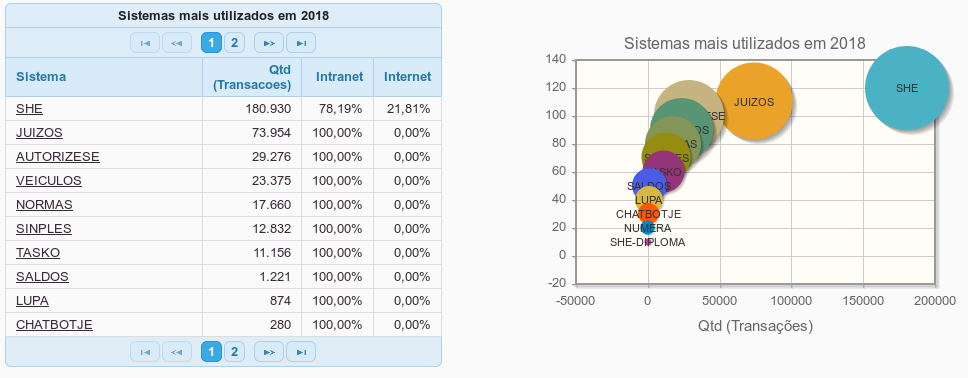
\includegraphics[width=0.75\textwidth]{./dados/figuras/ranking2018.png}
    \fonte{SEDES}
    \label{fig:figura-ranking2018}
\end{figure}

\begin{figure}[!htb]
    \centering
    \caption{Veículos - Ranking 2019}
    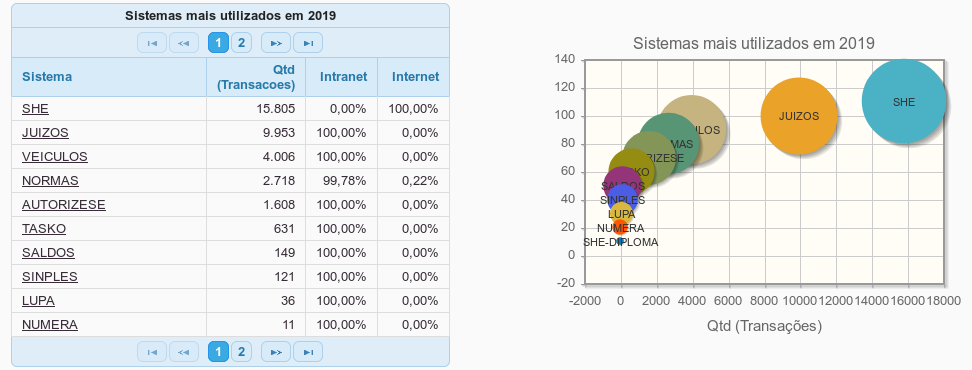
\includegraphics[width=0.75\textwidth]{./dados/figuras/ranking2019.png}
    \fonte{SEDES}
    \label{fig:figura-ranking2019}
\end{figure}

Nesse relatório serão explanados, tanto os conhecimentos teóricos, quanto os práticos, descrevendo todas as etapas do projeto. Também estarão presentes neste relatório informações referentes à empresa e sobre a unidade da empresa onde o projeto foi executado, além de informações sobre infra-estrutura.
Por fim, serão mencionadas as correlações entre o conteúdo visto em sala de aula e o que foi feito na prática, bem como as principais dificuldades encontradas durante a execução do projeto.


\section{Objetivo}
\label{sec:objetivo}

\subsection{Objetivo geral}
\label{sec:objetivoGeral}
Auxiliar no desenvolvimento dos ativos, soluções web desenvolvidas pela SEDES, participando de todas as atividades contempladas pelas etapas descritas no Modelo de Desenvolvimento de Software adotado pelo TRE-PB.  Para vistas deste relatório será utilizado como referência o projeto \imprimirtitulo. O sistema deve ser capaz de receber solicitações dos usuários e exibi-las em um painel onde o gestor deverá analisar os pedidos e montar as viagens adequando: rotas, disponibilidades dos motoristas e passageiros.

\subsection{Objetivos específicos}
\label{sec:objetivosEspecificos}
Contribuir na implementação do Sistema de Gestão de Frotas, quando possível oferecendo alternativas para a implementação mediante aos conhecimentos adquiridos na graduação. Ganhar experiência com o fluxo de trabalho da uma equipe de desenvolvimento incorporando conceitos de metodologias ágeis e versionamento de código, sendo capaz de resolver conflitos de códigos, quando houver, e evita-los. Trabalhar com reuniões diárias, planejar soluções com a modelagem do negócio especificando suas respectivas histórias de usuários, codificar utilizando as tecnologias e padrões adotados pela equipe, realizar entregas frequentes sempre buscando feedback das releases pelo cliente e gerar documentação explicando as funcionalidades e como utiliza-las. 

% utilizar met. ágeis, trabalhar em equipe, participar de reuniões, documentar, especificar, implementar...

\section{A Empresa}\footnote{http://www.tre-pb.jus.br/institucional/conheca-o-tre-pb/conheca-o-tre-pb}
\label{sec:empresa}
A Justiça Eleitoral é o ramo especializado do Poder Judiciário que visa garantir a lisura, a eficiência e a eficácia do processo eleitoral, contribuindo para o fortalecimento da democracia e a consolidação do Estado de Direito. Compete à Justiça Eleitoral preparar, realizar e apurar as eleições, além de administrar o Cadastro Nacional de Eleitores.
O principal objetivo da Justiça Eleitoral é o gerenciamento do processo eleitoral, através de diretrizes claras e firmes, evitando vícios, abusos e fraudes.
O Tribunal Regional Eleitoral da Paraíba - TRE-PB, órgão máximo da Justiça Eleitoral no Estado, tem como instância superior, em matéria eleitoral, o Tribunal Superior Eleitoral, sediado em Brasília - Distrito Federal. A finalidade do TRE-PB é planejar e coordenar o processo eleitoral nas eleições federais, estaduais e municipais, no âmbito do Estado da Paraíba.
Compete, também, ao Tribunal, julgar os recursos interpostos das decisões dos Juízes e Juntas Eleitorais do Estado, bem como, os processos originários e administrativos do próprio Tribunal; registrar os partidos e candidatos a cargos eletivos de Governador, Senador, Deputado Federal e Estadual, assim como, receber e analisar a prestação de contas dos mesmos, prestadas ao final de cada campanha estadual; analisar as prestações de contas anuais dos órgãos regionais dos partidos políticos; elaborar e fiscalizar o calendário estadual de propaganda eleitoral; proceder à anotação e cancelamento dos diretórios estaduais e municipais dos partidos políticos; julgar as impugnações relativas aos pedidos de registros de candidaturas e as arguições de inelegibilidade; designar os Juízes Titulares das Zonas Eleitorais do Estado da Paraíba e administrar o Cadastro de Eleitores.

\section{Descrição geral das atividades}
\label{sec:descricaoGeralAtividades}
Durante o processo foram utilizadas as metodologias Scrum para gestão e planejamento dos projetos e o Kanban para o controle de fluxo do desenvolvimento. As atividades desenvolvidas no período do estágio foram as seguintes de acordo com as fases: 
\begin{enumerate}
    \item Imersão:
    \begin{enumerate}
        \item Elicitação das histórias de usuário.
        \item Definição do escopo do produto.
        \item Criar estrutura do projeto.
        \item Modelagem de dados.
    \end{enumerate}
   \item Construção:
   \begin{enumerate}
        \item Refinar histórias de usuário.
        \item Estimar histórias.
        \item Codificação de funcionalidades.
        \item Preparar versão para homologação.
        \item Codificar ajustes.
        \item Gerar documentação.
        \item Implantar versão.
   \end{enumerate}
\end{enumerate}

\section{Organização do relatório}
\label{sec:organizacaoRelatorio}
Além desse capítulo, o relatório está dividido em outros três capítulos brevemente descritos abaixo:

\autoref{chap:embasamentoTeorico} - Embasamento Teórico: aborda as tecnologias e linguagens que foram utilizadas durante o estágio, bem como as definições necessárias para a compreensão do processo.

\autoref{chap:atividadesRealizadas} - Atividades Realizadas: apresenta o projeto, no qual as atividades do estagiário foram realizadas, descrevendo os principais conceitos e funcionalidades. Relata as atividades realizadas ao longo do período de estágio descrevendo o fluxo e o processo de desenvolvimento e detalha a implementação de algumas funcionalidades.

\autoref{chap:consideracoesFinais} – Considerações Finais: Apresenta um relato sobre as experiências adquiridas, metas e objetivos alcançados. O quão grande foi a contribuição do estágio na minha formação profissional.
